\documentclass[11pt,letterpaper]{article}
\usepackage[utf8]{inputenc}
\usepackage[left=1in,right=1in,top=1in,bottom=1in]{geometry}
\usepackage{amsfonts,amsmath}
\usepackage{graphicx,float}
% -----------------------------------
\usepackage{hyperref}
\hypersetup{%
  colorlinks=true,
  linkcolor=blue,
  citecolor=blue,
  urlcolor=blue,
  linkbordercolor={0 0 1}
}
% -----------------------------------
\usepackage[style=authoryear-icomp,backend=biber]{biblatex}
\addbibresource{citation.bib}
% -----------------------------------
\usepackage{fancyhdr}
\newcommand\course{MATH-UA.0252\\Numerical Analysis}
\newcommand\hwnumber{7}                  % <-- homework number
\newcommand\NetIDa{Ryan Sh\`iji\'e D\`u} 
\newcommand\NetIDb{October 27th, 2023}
\pagestyle{fancyplain}
\headheight 35pt
\lhead{\NetIDa\\\NetIDb}
\chead{\textbf{\Large Worksheet \hwnumber}}
\rhead{\course}
\lfoot{}
\cfoot{}
\rfoot{\small\thepage}
\headsep 1.5em
% -----------------------------------
\usepackage{titlesec}
\renewcommand\thesubsection{(\arabic{section}.\alph{subsection})}
\titleformat{\subsection}[runin]
        {\normalfont\bfseries}
        {\thesubsection}% the label and number
        {0.5em}% space between label/number and subsection title
        {}% formatting commands applied just to subsection title
        []% punctuation or other commands following subsection title
% -----------------------------------
\setlength{\parindent}{0.0in}
\setlength{\parskip}{0.1in}
% -----------------------------------
\newcommand{\de}{\mathrm{d}}
\newcommand{\DD}{\mathrm{D}}
\newcommand{\pe}{\partial}
\newcommand{\mcal}{\mathcal}
%\newcommand{\pdx}{\left|\frac{\partial}{\partial_x}\right|}

\newcommand{\dsp}{\displaystyle}

\newcommand{\norm}[1]{\left\Vert #1 \right\Vert}
%\newcommand{\mean}[1]{\left\langle #1 \right\rangle}
\newcommand{\mean}[1]{\overline{#1}}
\newcommand{\inner}[2]{\left\langle #1,#2\right\rangle}

\newcommand{\ve}[1]{\boldsymbol{#1}}

\newcommand{\thus}{\Rightarrow \quad }
\newcommand{\fff}{\iff\quad}
\newcommand{\qdt}[1]{\quad \mbox{#1} \quad}

\renewcommand{\Re}{\mathrm{Re}}
\renewcommand{\Im}{\mathrm{Im}}
\newcommand{\E}{\mathbb{E}}
\newcommand{\lap} {\nabla^2}
\renewcommand{\div}{\nabla\cdot}

\newcommand{\csch}{\text{csch}}
\newcommand{\sech}{\text{sech}}


\newcommand{\hot}{\text{h.o.t.}}

\newcommand{\ssp}{\left.\qquad\right.}

\newcommand{\var}{\text{var}}
\newcommand{\cov}{\text{cov}}

%%%%%%%%%%%%%%%%%%%%%%%%%%%%%%%%%%%%%%%%%%%%%%%%%%
\makeatletter
\newcommand*{\mint}[1]{%
  % #1: overlay symbol
  \mint@l{#1}{}%
}
\newcommand*{\mint@l}[2]{%
  % #1: overlay symbol
  % #2: limits
  \@ifnextchar\limits{%
    \mint@l{#1}%
  }{%
    \@ifnextchar\nolimits{%
      \mint@l{#1}%
    }{%
      \@ifnextchar\displaylimits{%
        \mint@l{#1}%
      }{%
        \mint@s{#2}{#1}%
      }%
    }%
  }%
}
\newcommand*{\mint@s}[2]{%
  % #1: limits
  % #2: overlay symbol
  \@ifnextchar_{%
    \mint@sub{#1}{#2}%
  }{%
    \@ifnextchar^{%
      \mint@sup{#1}{#2}%
    }{%
      \mint@{#1}{#2}{}{}%
    }%
  }%
}
\def\mint@sub#1#2_#3{%
  \@ifnextchar^{%
    \mint@sub@sup{#1}{#2}{#3}%
  }{%
    \mint@{#1}{#2}{#3}{}%
  }%
}
\def\mint@sup#1#2^#3{%
  \@ifnextchar_{%
    \mint@sup@sub{#1}{#2}{#3}%
  }{%
    \mint@{#1}{#2}{}{#3}%
  }%
}
\def\mint@sub@sup#1#2#3^#4{%
  \mint@{#1}{#2}{#3}{#4}%
}
\def\mint@sup@sub#1#2#3_#4{%
  \mint@{#1}{#2}{#4}{#3}%
}
\newcommand*{\mint@}[4]{%
  % #1: \limits, \nolimits, \displaylimits
  % #2: overlay symbol: -, =, ...
  % #3: subscript
  % #4: superscript
  \mathop{}%
  \mkern-\thinmuskip
  \mathchoice{%
    \mint@@{#1}{#2}{#3}{#4}%
        \displaystyle\textstyle\scriptstyle
  }{%
    \mint@@{#1}{#2}{#3}{#4}%
        \textstyle\scriptstyle\scriptstyle
  }{%
    \mint@@{#1}{#2}{#3}{#4}%
        \scriptstyle\scriptscriptstyle\scriptscriptstyle
  }{%
    \mint@@{#1}{#2}{#3}{#4}%
        \scriptscriptstyle\scriptscriptstyle\scriptscriptstyle
  }%
  \mkern-\thinmuskip
  \int#1%
  \ifx\\#3\\\else_{#3}\fi
  \ifx\\#4\\\else^{#4}\fi  
}
\newcommand*{\mint@@}[7]{%
  % #1: limits
  % #2: overlay symbol
  % #3: subscript
  % #4: superscript
  % #5: math style
  % #6: math style for overlay symbol
  % #7: math style for subscript/superscript
  \begingroup
    \sbox0{$#5\int\m@th$}%
    \sbox2{$#5\int_{}\m@th$}%
    \dimen2=\wd0 %
    % => \dimen2 = width of \int
    \let\mint@limits=#1\relax
    \ifx\mint@limits\relax
      \sbox4{$#5\int_{\kern1sp}^{\kern1sp}\m@th$}%
      \ifdim\wd4>\wd2 %
        \let\mint@limits=\nolimits
      \else
        \let\mint@limits=\limits
      \fi
    \fi
    \ifx\mint@limits\displaylimits
      \ifx#5\displaystyle
        \let\mint@limits=\limits
      \fi
    \fi
    \ifx\mint@limits\limits
      \sbox0{$#7#3\m@th$}%
      \sbox2{$#7#4\m@th$}%
      \ifdim\wd0>\dimen2 %
        \dimen2=\wd0 %
      \fi
      \ifdim\wd2>\dimen2 %
        \dimen2=\wd2 %
      \fi
    \fi
    \rlap{%
      $#5%
        \vcenter{%
          \hbox to\dimen2{%
            \hss
            $#6{#2}\m@th$%
            \hss
          }%
        }%
      $%
    }%
  \endgroup
}

\begin{document} 

\section{Geometric interpretation of Householder reflectors}
\subsection{}
Name $H(\ve v)$ the linear subspace orthogonal to the vector $\ve v$. A reflector across $H(\ve v)$ is 
\begin{align*}
    F_{\ve v} = I - 2 \frac{\ve v \ve v^\top}{\ve v^\top \ve v}.
\end{align*}
Compare this with $P_v$ and $P_{\perp v}$, and interpret the formula geometrically.

\begin{figure}[H]
    \centering
    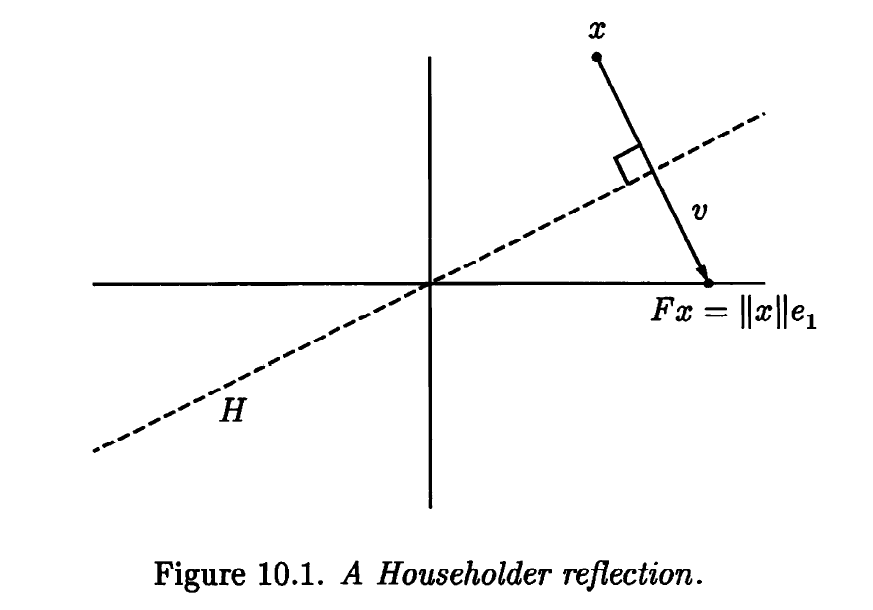
\includegraphics[width = 0.6\textwidth]{Session_7/latex/figs/TB_HouseholderRef}
\end{figure}

\subsection{}
To use Householder for QR decomposition, we want $F\ve x = c\ve e_1$. We know that $c = \pm\norm{\ve x}_2$. Explain this geometrically.

\subsection{}
From this, we have that
\begin{align*}
    \ve v = \ve x- F\ve x =  \ve x \pm \norm{\ve x}\ve e_1.
\end{align*}
From a geometric point of view, why is this the correct formula?

\section{Gershgorin disks and the power method}
Consider the matrix 
$$
A = \begin{bmatrix}
- 6 & 2 & 0.3 & 0 & -0.7 \\
2 & - 4 & 0.1 & 0.05 & 0 \\
0.3 & 0.1 & 2 & 0.1 & 0.1 \\
0 & 0.05 & 0.1 &  4 & 0 \\
-0.7 & 0 & 0.1  & 0  & 6
\end{bmatrix}
$$
and recall the definition of the Gershgorin disks:
\[
D_i = \{ z \in \mathbb C ~|~ |z - a_{ii}| \le \sum_{j \ne i} |a_{ij}| \}.
\]

\subsection{}
Argue that all eigenvalues of $A$ are real.

\subsection{}
What are the Gershgorin disks for $A$?  Use them to give a set, $D \subset \mathbb{R}$, that contains all eigenvalues of $A$.

\subsection{}
Can you conclude that the eigenvalue with the largest absolute value is simple?

\subsection{}
Argue that $A$ is invertible. Conclude that all diagonally dominant matrix is invertible.

\subsection{}
True or False? Let $A \in \mathbb{R}^{n \times n}$ and $D_i$, $i
  = 1,2,\dots,n$, be the Gerschgorin disks of $A$. If $0 \in
  \bigcup_{i=1}^n D_i$ then $A$ is singular.
  
\subsection{}
Write down the first iteration of the power method starting from $\ve x_0 = (0,0,0,0,1)^T$.
You don't need to normalize.
Explain why $\ve x_0 = \ve 0$ is not a suitable starting point.

\subsection{}
The eigenvalues of $A$, after rounding, are $\{-7, -3, 2, 4, 6\}$.
Which eigenvalue direction will the sequence of the previous question converge to?

\section{Eigenvectors as stationary points of Rayleigh quotient}
For $H$ a real symmetric matrix, we define Rayleigh quotient as a function $\mathbb{R}^n\to\mathbb{R}$:
\begin{align*}
    R(\ve x) = \frac{\ve x^\top H\ve x}{\ve x^\top \ve x} = \frac{q(\ve x)}{p(\ve x)}.
\end{align*}
We will show that $\ve v$ is a stationary point (i.e.: $\nabla R(\ve v) = 0$) of the Rayleigh quotient if and only if it is an eigenvector of $H$ (cf. \cite[p.114-116]{Lax_07} and \cite[p.203-204]{TrefethenBau_97}).

\subsection{}
To characterize a point such that $\nabla R(\ve v) = 0$, we need to know the gradient of $R(\ve x)$ at $\ve v$. We could do this, but an alternative approach is to take $t\in \mathbb{R}$ and calculate
\begin{align*}
    \left.\frac{\de}{\de t} R(\ve v+t\ve y)\right|_{t=0}
\end{align*}
for all $\ve y\in\mathbb{R}^n$. In particular, we can get the gradient by picking $\ve y = \ve e_i$.

\subsection{}
Using the above calculation, show the iff claim in the main text of the problem.

    
\printbibliography

\end{document}